\chapter*{Annexes}
\addcontentsline{toc}{chapter}{Annexes}
\markboth{Annexes}{}
\stepcounter{chapter}
\addtocontents{lot}{\vspace{3.8mm}}
\addtocontents{lof}{\vspace{3.8mm}}

%Mettez vos annexes ici...

%===================== ANNEXE 1 =====================%
\section*{Annexe 1.~L'algorigramme de «mise à jour des données boutiques»}
\addcontentsline{toc}{section}{Annexe 1.~L'algorigramme de «mise à jour des données boutiques»}
Ce diagramme représente l'algorithme de script bash qui s'exécute quotidiennement pour mettre à jour les données boutiques.
\begin{figure}[H]
	\centering
	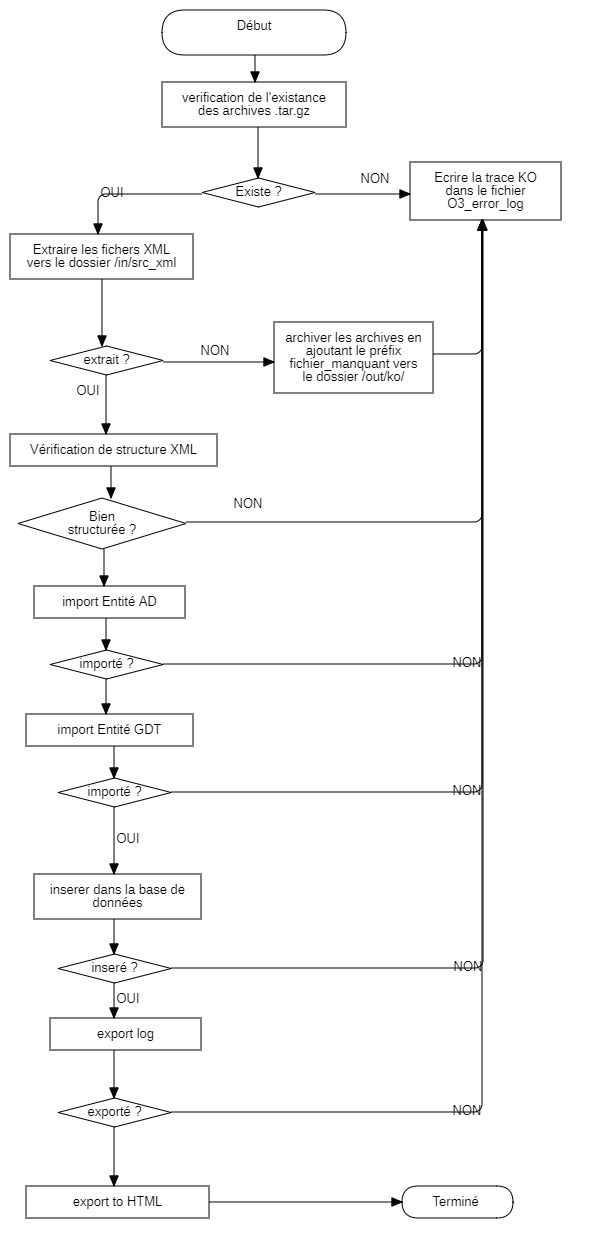
\includegraphics[width=0.5\linewidth]{img/conception/FlowchartDiagram-update-boutique}
	\caption[L'algorigramme de «mise à jour des données boutiques»]{L'algorigramme de «mise à jour des données boutiques»}
	\label{fig:flowchartdiagram-update-boutique}
\end{figure}
\newpage
%===================== ANNEXE 2 =====================%
\section*{Annexe 2.~Extrait des fichier XML}
\addcontentsline{toc}{section}{Annexe 2.~Extrait des fichier XML}

\addcontentsline{lof}{figure}{Annexe 2.1~~~Extrait des fichiers XML de mise à jour de données boutique}

La figure annexe 2.1 présente un extrait des fichiers XML de mise à jour de données boutique.
\begin{figure}[htpb]
    \centering
    \frame{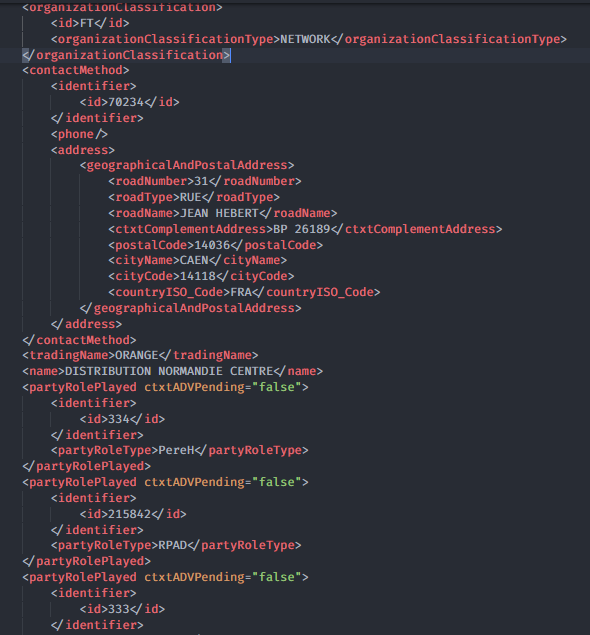
\includegraphics[width=0.7\columnwidth]{/extraitxml}}
    {\\\textbf{Figure annexe 2.1:} Extrait des 0fichiers XML de mise à jour de données boutique}
\end{figure}\newpage
%===================== ANNEXE 3 =====================%
\section*{Annexe 3.~Dictionnaire de données}
\addcontentsline{toc}{section}{Annexe 3.~Dictionnaire de données}

\addcontentsline{lof}{figure}{Annexe 3.1~~~Dictionnaire de données}

Le tableau annexe 3.1 présente le dictionnaire de données.\\
\begin{longtable}[c]{|c|l|l|}
	\hline
	\rowcolor[HTML]{C0C0C0} 
	\multicolumn{1}{|l|}{\cellcolor[HTML]{C0C0C0}Classes} & colonnes     & signification                              \\ \hline
	\endhead
	%
	& {\ul \textbf{id\_user}}   & identifiant de l'utilisateur               \\ \cline{2-3} 
	& username                  & identifiant Orange (CUID)                  \\ \cline{2-3} 
	& typeUser                  & identifiant de type                        \\ \cline{2-3} 
	& password                  & mot de passe de l'utilisateur              \\ \cline{2-3} 
	& salt                      & utilisé pour le hashage de mot de passe    \\ \cline{2-3} 
	& token                     &                                            \\ \cline{2-3} 
	& token\_date               &                                            \\ \cline{2-3} 
	& active                    & activation de l'utilisateur                \\ \cline{2-3} 
	& preferred\_language       & langue préférée de l'utilisateur           \\ \cline{2-3} 
	& civility                  & civilité                                   \\ \cline{2-3} 
	& interne                   & utilisateur Orange ou pas                  \\ \cline{2-3} 
	& givenname                 & nom de l'utilisateur                       \\ \cline{2-3} 
	& surname                   & prénom de l'utilisateur                    \\ \cline{2-3} 
	& mail                      & email de l'utilisateur                     \\ \cline{2-3} 
	& entity                    & entité à laquelle appartient l'utilisateur \\ \cline{2-3} 
	& creation\_date            & date de création                           \\ \cline{2-3} 
	& update\_date              & derniere date de mise à jour               \\ \cline{2-3} 
	& start\_date\_activation   & date d'activation de compte                \\ \cline{2-3} 
	& end\_date\_activation     & date de fin d'utilisation de compte        \\ \cline{2-3} 
	\multirow{-20}{*}{\textbf{User}}                      & action       & action lors l'importation de fichier Excel \\ \hline
	& id\_acl\_role             & identifiant de role                        \\ \cline{2-3} 
	& name                      & court nom de role                          \\ \cline{2-3} 
	& fullname                  & nom complet de role                        \\ \cline{2-3} 
	& start\_date\_activate\_ra & date d'activation de role                  \\ \cline{2-3} 
	& end\_date\_activate\_ra   & date de fin d'utilisation de role          \\ \cline{2-3} 
	& enabled                   & activation de role                         \\ \cline{2-3} 
	& created\_at               & date de création                           \\ \cline{2-3} 
	\multirow{-8}{*}{\textbf{Roles}}                      & update\_time & derniere date de mise à jour               \\ \hline
	& active                    & activation                                 \\ \cline{2-3} 
	\multirow{-2}{*}{\textbf{user-role}} & created\_at               & date de création                           \\ \hline
	& {\ul \textbf{id\_type}}   & identifiant de type                        \\ \cline{2-3} 
	\multirow{-2}{*}{\textbf{Type}}      & type                      & libellé de type (3901, CPRO)               \\ \hline
	\captionsetup{justification=centering}
	\caption{Dictionnaire de données 1}
	\label{tab:dictio-1}\\
\end{longtable}
\newpage
% Please add the following required packages to your document preamble:
% \usepackage{multirow}
% \usepackage[table,xcdraw]{xcolor}
% If you use beamer only pass "xcolor=table" option, i.e. \documentclass[xcolor=table]{beamer}
% \usepackage[normalem]{ulem}
% \useunder{\uline}{\ul}{}
% \usepackage{longtable}
% Note: It may be necessary to compile the document several times to get a multi-page table to line up properly
\begin{longtable}[c]{|c|l|l|}
	\hline
	\rowcolor[HTML]{C0C0C0} 
	\multicolumn{1}{|l|}{\cellcolor[HTML]{C0C0C0}Classes}  & colonnes     & signification                       \\ \hline
	\endhead
	%
	& {\ul \textbf{code\_edo}} & identifiant boutique              \\ \cline{2-3} 
	& libelle\_edo & libellé boutique ( nom commercial ) \\ \cline{2-3} 
	& sous\_canal              & marché client                     \\ \cline{2-3} 
	& type\_edo                & type de boutique                  \\ \cline{2-3} 
	& sous\_type               & Point de vente ou Boutique Orange \\ \cline{2-3} 
	& status                   & activation                        \\ \cline{2-3} 
	& designation              & nom complet de boutique           \\ \cline{2-3} 
	& num\_voie                & numero des voies                  \\ \cline{2-3} 
	& type\_voie               & type de voie                      \\ \cline{2-3} 
	& nom\_voie                & nom de voie                       \\ \cline{2-3} 
	& code\_postal             & code postal de boutique           \\ \cline{2-3} 
	& ville                    & ville de boutique                 \\ \cline{2-3} 
	\multirow{-13}{*}{\textbf{Boutique}}                   & pays         & pays de boutique                    \\ \hline
	Boutique                        & email                    & email de contact de boutique      \\ \hline
	& {\ul \textbf{id}}        & identifiant de l'affectation      \\ \cline{2-3} 
	\multirow{-2}{*}{\textbf{affectation\_user\_boutique}} & created\_at  & date d'affectation                  \\ \hline
	& {\ul \textbf{id}}        & identifiant de l'application      \\ \cline{2-3} 
	& basicat                  & code application                  \\ \cline{2-3} 
	& url\_dev                 & adresse de serveur developpement  \\ \cline{2-3} 
	& url\_qualif              & adresse de serveur qualification  \\ \cline{2-3} 
	& url\_preprod             & adresse de serveur préproduction  \\ \cline{2-3} 
	& url\_prod                & adresse de serveur production     \\ \cline{2-3} 
	& url\_int                 & adresse de serveur d'intégration  \\ \cline{2-3} 
	& name                     & nom application                   \\ \cline{2-3} 
	& encoding                 & encodage                          \\ \cline{2-3} 
	& type                     & type (externe, panoramix)         \\ \cline{2-3} 
	& description              & description de l'application      \\ \cline{2-3} 
	\multirow{-12}{*}{\textbf{application}}                & update\_time & derniere date de mise à jour        \\ \hline
	& id                       & identifiant de pef                \\ \cline{2-3} 
	& pef\_name                & nom court de pef                  \\ \cline{2-3} 
	& pef\_libelle             & nom complet de pef                \\ \cline{2-3} 
	& tab\_libelle             & nom de fenetre                    \\ \cline{2-3} 
	& url                      & adresse de pef                    \\ \cline{2-3} 
	& url\_methode             & adresse de methode                \\ \cline{2-3} 
	& call\_methode            & methode d'appel                   \\ \cline{2-3} 
	& unique\_tab              &                                   \\ \cline{2-3} 
	& confirme\_open\_id       &                                   \\ \cline{2-3} 
	& stat                     & activation                        \\ \cline{2-3} 
	& context                  & contexte                          \\ \cline{2-3} 
	& delegatable              &                                   \\ \cline{2-3} 
	& type\_mapping            &                                   \\ \cline{2-3} 
	& callback                 &                                   \\ \cline{2-3} 
	& iframe\_title            & titre de l'iframe                 \\ \cline{2-3} 
	& id\_categorie            & catégorie de pef                  \\ \cline{2-3} 
	& output\_show             & faire des outputs ou noon         \\ \cline{2-3} 
	& update\_time             & derniere date de mise à jour      \\ \cline{2-3} 
	\multirow{-19}{*}{\textbf{PEF}} & canal                    &                                   \\ \hline
	\captionsetup{justification=centering}
	\caption{Dictionnaire de données 2}
	\label{tab:dictio-2}\\
\end{longtable}

\newpage

\begin{longtable}[c]{|c|l|l|}
	\hline
	\rowcolor[HTML]{C0C0C0} 
	\multicolumn{1}{|l|}{\cellcolor[HTML]{C0C0C0}Classes} & colonnes          & signification                          \\ \hline
	\endhead
	%
	& {\ul \textbf{id}} & identifiant de catégorie d'application \\ \cline{2-3} 
	& name              & libellé de catégorie                   \\ \cline{2-3} 
	& ordre\_affichage  & odre d'affichage                       \\ \cline{2-3} 
	\multirow{-4}{*}{\textbf{Categorie}}                  & update\_time      & derniere date de mise à jour           \\ \hline
	\captionsetup{justification=centering}
	\caption{Dictionnaire de données 3}
	\label{tab:dictio-3}\\
\end{longtable}